
%(BEGIN_QUESTION)
% Copyright 2010, Tony R. Kuphaldt, released under the Creative Commons Attribution License (v 1.0)
% This means you may do almost anything with this work of mine, so long as you give me proper credit

An antimicrobial agent called {\it acrolein} used to protect diesel fuel from fungal growth may be manufactured by reacting propylene with steam and air in a reactor vessel: 

$$\includegraphics[width=15.5cm]{i00735x01.eps}$$

Suppose operators call you to troubleshoot a problem they are having with this process, and to help you start they show you this graphic display on one of their DCS workstations.  Identify the problem in this process, suggest at least two possible causes for it, and identify the next diagnostic step you would take to confirm the cause(s).

\vskip 20pt \vbox{\hrule \hbox{\strut \vrule{} {\bf Suggestions for Socratic discussion} \vrule} \hrule}

\begin{itemize}
\item{} Identify a good troubleshooting strategy to apply to a control system graphic such as this, to quickly {\it identify which part of the system} is experiencing trouble.
\end{itemize}

\underbar{file i00735}
%(END_QUESTION)





%(BEGIN_ANSWER)

The problem here is that steam flow controller FC-188 is having trouble maintaining setpoint.  I'll let you figure out possible causes for this problem.

%(END_ANSWER)





%(BEGIN_NOTES)

Either there is very little HP steam flow into the reactor (despite the controller trying to increase flow with a wide-open valve), or the transmitter is falsely indicating a very low flow rate.  The abnormally low HP steam header pressure (30 PSI) is barely above the reactor pressure, which would support a conclusion of very little flow through the control valve despite the valve being wide-open.  The problem most likely lies with the steam system (not supplying enough pressure to this acrolein process).

A good ``next step'' would be to switch to another page on the DCS display and monitor parameters associated with steam production and distribution.  Perhaps the boilerhouse is having process problems, or someone pinched off a hand-operated steam valve?

%INDEX% Process: acrolein production 
%INDEX% Process troubleshooting: diagnosing problem via DCS display

%(END_NOTES)


